\documentclass{standalone}
\usepackage{tikz}
\usepackage{ctex}
\setCJKmainfont{Noto Serif CJK SC}
\usepackage{mhchem,siunitx}
\usetikzlibrary{patterns,patterns.meta}
\begin{document}
\small
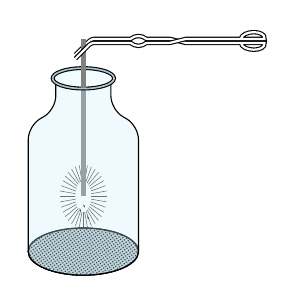
\begin{tikzpicture}[>=stealth,scale=1.0,inner sep=2pt]
  \draw[double distance=0.8pt,rounded corners=1pt](-0.1,1.3)--++(0.2,0.2)[sharp corners]--++(0.5,0)to[bend left=40](0.8,1.5)--++(0.3,0)--++(0.2,-0.05)--++(1.0,0)to[out=-80,in=-80](2.0,1.45);
  \foreach \x in {10,20,...,360}
  {
    \draw[very thin,darkgray]({0.1*cos(\x)},{0.2*sin(\x)-0.5})--({0.3*cos(\x)},{0.4*sin(\x)-0.5});
  }
  \fill(0,-0.6)to[in=-160,out=-90](0.02,-0.64)to[out=20](0,-0.6);
  \fill(-0.05,-0.65)to[in=-160,out=-90](-0.03,-0.69)to[out=20](-0.05,-0.65);
  \fill(0.05,-0.75)to[in=-160,out=-90](0.07,-0.79)to[out=20](0.05,-0.75);
  \draw[ultra thick,gray](0,0.86)--(0,-0.5);
  \draw[fill=cyan!10!lightgray](0,-1.2)ellipse(0.7 and 0.3);
  \draw[pattern={Dots[angle=35,radius=0.3pt,distance=1pt]}](0,-1.2)ellipse(0.7 and 0.3);
  
  \draw[rounded corners=5pt,fill=cyan!20!white,fill opacity=0.3](0.35,1.0)--(0.35,0.6)--(0.7,0.4)[sharp corners]--(0.7,-1.2)arc(0:-180:0.7 and 0.3)[rounded corners=5pt]--(-0.7,0.4)--(-0.35,0.6)--(-0.35,1.0);
  \draw[double=cyan!20!lightgray,fill=cyan!5!white](0,1.0)ellipse(0.39 and 0.13);
  \draw[ultra thick,gray](0,0.88)--(0,1.5);
  \draw[double distance=0.8pt,rounded corners=1pt](-0.1,1.25)--++(0.2,0.2)[sharp corners]--++(0.5,0)to[bend right=40](0.8,1.45)--++(0.3,0)--++(0.2,0.05)--++(1.0,0)to[out=80,in=80](2.0,1.5);

\end{tikzpicture}
\end{document}